\documentclass[]{elsarticle} %review=doublespace preprint=single 5p=2 column
%%% Begin My package additions %%%%%%%%%%%%%%%%%%%
\usepackage[hyphens]{url}

  \journal{An awesome journal} % Sets Journal name


\usepackage{lineno} % add
\providecommand{\tightlist}{%
  \setlength{\itemsep}{0pt}\setlength{\parskip}{0pt}}

\usepackage{graphicx}
\usepackage{booktabs} % book-quality tables
%%%%%%%%%%%%%%%% end my additions to header

\usepackage[T1]{fontenc}
\usepackage{lmodern}
\usepackage{amssymb,amsmath}
\usepackage{ifxetex,ifluatex}
\usepackage{fixltx2e} % provides \textsubscript
% use upquote if available, for straight quotes in verbatim environments
\IfFileExists{upquote.sty}{\usepackage{upquote}}{}
\ifnum 0\ifxetex 1\fi\ifluatex 1\fi=0 % if pdftex
  \usepackage[utf8]{inputenc}
\else % if luatex or xelatex
  \usepackage{fontspec}
  \ifxetex
    \usepackage{xltxtra,xunicode}
  \fi
  \defaultfontfeatures{Mapping=tex-text,Scale=MatchLowercase}
  \newcommand{\euro}{€}
\fi
% use microtype if available
\IfFileExists{microtype.sty}{\usepackage{microtype}}{}
\bibliographystyle{elsarticle-harv}
\ifxetex
  \usepackage[setpagesize=false, % page size defined by xetex
              unicode=false, % unicode breaks when used with xetex
              xetex]{hyperref}
\else
  \usepackage[unicode=true]{hyperref}
\fi
\hypersetup{breaklinks=true,
            bookmarks=true,
            pdfauthor={},
            pdftitle={Using Plumber to Create a Distributed Modeling Framework for Protected Data},
            colorlinks=false,
            urlcolor=blue,
            linkcolor=magenta,
            pdfborder={0 0 0}}
\urlstyle{same}  % don't use monospace font for urls

\setcounter{secnumdepth}{0}
% Pandoc toggle for numbering sections (defaults to be off)
\setcounter{secnumdepth}{0}
% Pandoc header



\begin{document}
\begin{frontmatter}

  \title{Using Plumber to Create a Distributed Modeling Framework for Protected
Data}
    \author[Some Institute of Technology]{Alice Anonymous\corref{c1}}
   \ead{alice@example.com} 
   \cortext[c1]{Corresponding Author}
    \author[Another University]{Bob Security}
   \ead{bob@example.com} 
  
      \address[Some Institute of Technology]{Department, Street, City, State, Zip}
    \address[Another University]{Department, Street, City, State, Zip}
  
  \begin{abstract}
  This is the abstract.
  
  It consists of two paragraphs.
  \end{abstract}
  
 \end{frontmatter}

\hypertarget{introduction}{%
\section{Introduction}\label{introduction}}

Here we introduce a conceptual framework to analyze data from multiple
sources with the data being properly siloed.

The motivation for this problem is simple: we would like to fit a
statistical model on data from multiple hospitals, where the indvidual
patient-level data never leaves the server. The idea is that a model is
specified, and sent to each hospital where a summary statistic is
computed and returned to the modeler. The model is then updated and, if
necessary, the process is completed until the model is fully fit.

The alternative to this process is meta-analysis. There are drawbacks to
a meta-analysis approach in that the model and statistics must be
specified and commonly the data is gathered once from each hospital. Any
updated analysis requires additional correspondence between the modeler
and the hospital data person, which slows down the process of analysis
and creates more hurdles. If this process is automated through a system
such as the API described below, this alleviates the need for staff to
run the computations individually (which can cause errors). Moreover,
when a hospital no longer wants to participate in the modeling process,
they can simply shut off their server.

Chen et al.~describes these processes as one-shot or multi-shot
analyses.

\hypertarget{motivating-example}{%
\section{Motivating Example}\label{motivating-example}}

In the most simple modeling example, let us estimate a linear regression
of an outcome \(Y\) on a set of covariates \(X\). Let there be \(K\)
hospitals, and \(Y\) and \(X\) are on the data on all hospitals
\(1, \dots, K\).

\[
E[Y | X] = X\beta
\]

Let us also say that we are interested in \(p\) covariates, and
\(n_{k}\) is the total number of records at hospital \(k\) and
\(n = \sum_{1}^{k} n_{k}\), is the number of rows of \(Y\) and \(X\),
thus \(Y\) is an \(n\text{x}1\) vector and \(X\) is a \(n\text{x}p\)
matrix. To estimate \(\beta\), we would use: \[
(X'X)^{-1} X'Y
\] where \(X'X\) is a \(p\text{x}p\) matrix and \(X'Y\) is a
\(p\times{1}\) vector.

Since we don't have access to \(X\), but rather a series of \(X_{k}\),
\(k = 1, \dots, K\), we can use methods such as parallelized gradient
descent approaches (Mcdonald et al., 2009; Zinkevich et al., 2010) or
approximate maximum-likelihood approaches (Duncan, 1980). Regardless,
for almost any approach, the gradient or some reduced-dimensional
summary is required to be aggregated together to get the estimate of
\(\beta\) at the full population level. Now, if we combine these models
with models that require iterative fitting, such as Generalized Linear
Models (GLMs), there needs to be a lot of communication and
recomputation of summaries to get a final estimate. These approaches
work well in distributed computing systems (such as computing clusters
or GPUs), but have a much higher likelihood for errors if human
interaction is required at each iteration. This human interaction is a
common practice for most clinical data, which we wish to show a simple
solution to create the distributed computing much simpler.

\hypertarget{methods}{%
\section{Methods}\label{methods}}

\texttt{plumber} is an R package that creates APIs (Application
programming interfaces) for and from R (Trestle Technology, LLC, 2018).
Though there are many frameworks to create APIs, such as Node.js and
Flask, we will focus on \texttt{plumber} for a number of reasons.
Overall, the API needs a computational backbone for this process to
work. As \texttt{plumber} is based in R, we know that the server will
have this already installed. Another reason is that the statisticians
and data analysts that will be running the models will likely be using a
statistical language, usually either R or Python. Though we will focus
on R, the ideas here can be extended to other languages and systems. We
are not experts in distributed computing, but would like to show how
this process is possible, overlooking obvious hurdles such as
authentication, load balancing, network issues, debugging, and overall
security on the server side.

The framework is as follows: a developer makes an R package with a
\texttt{plumber} API specification inside of it of the inputs and
outputs necessary for a specific model. For example, fitting a linear
model where the analyst specifies predictors and an outcome. The API has
endpoints that take in this model, run a specified computation on the
server (behind the hospital firewall), and returns a result that has
only aggregate data (such as a \(p\text{x}p\) matrix). The API logs the
output for potential future debugging and audits of the process. The
analysis system receives the output for each hospital, creates and
updated estimate of the model and runs the next iteration from each
hospital again until convergence. Thus, this system.

\begin{figure}
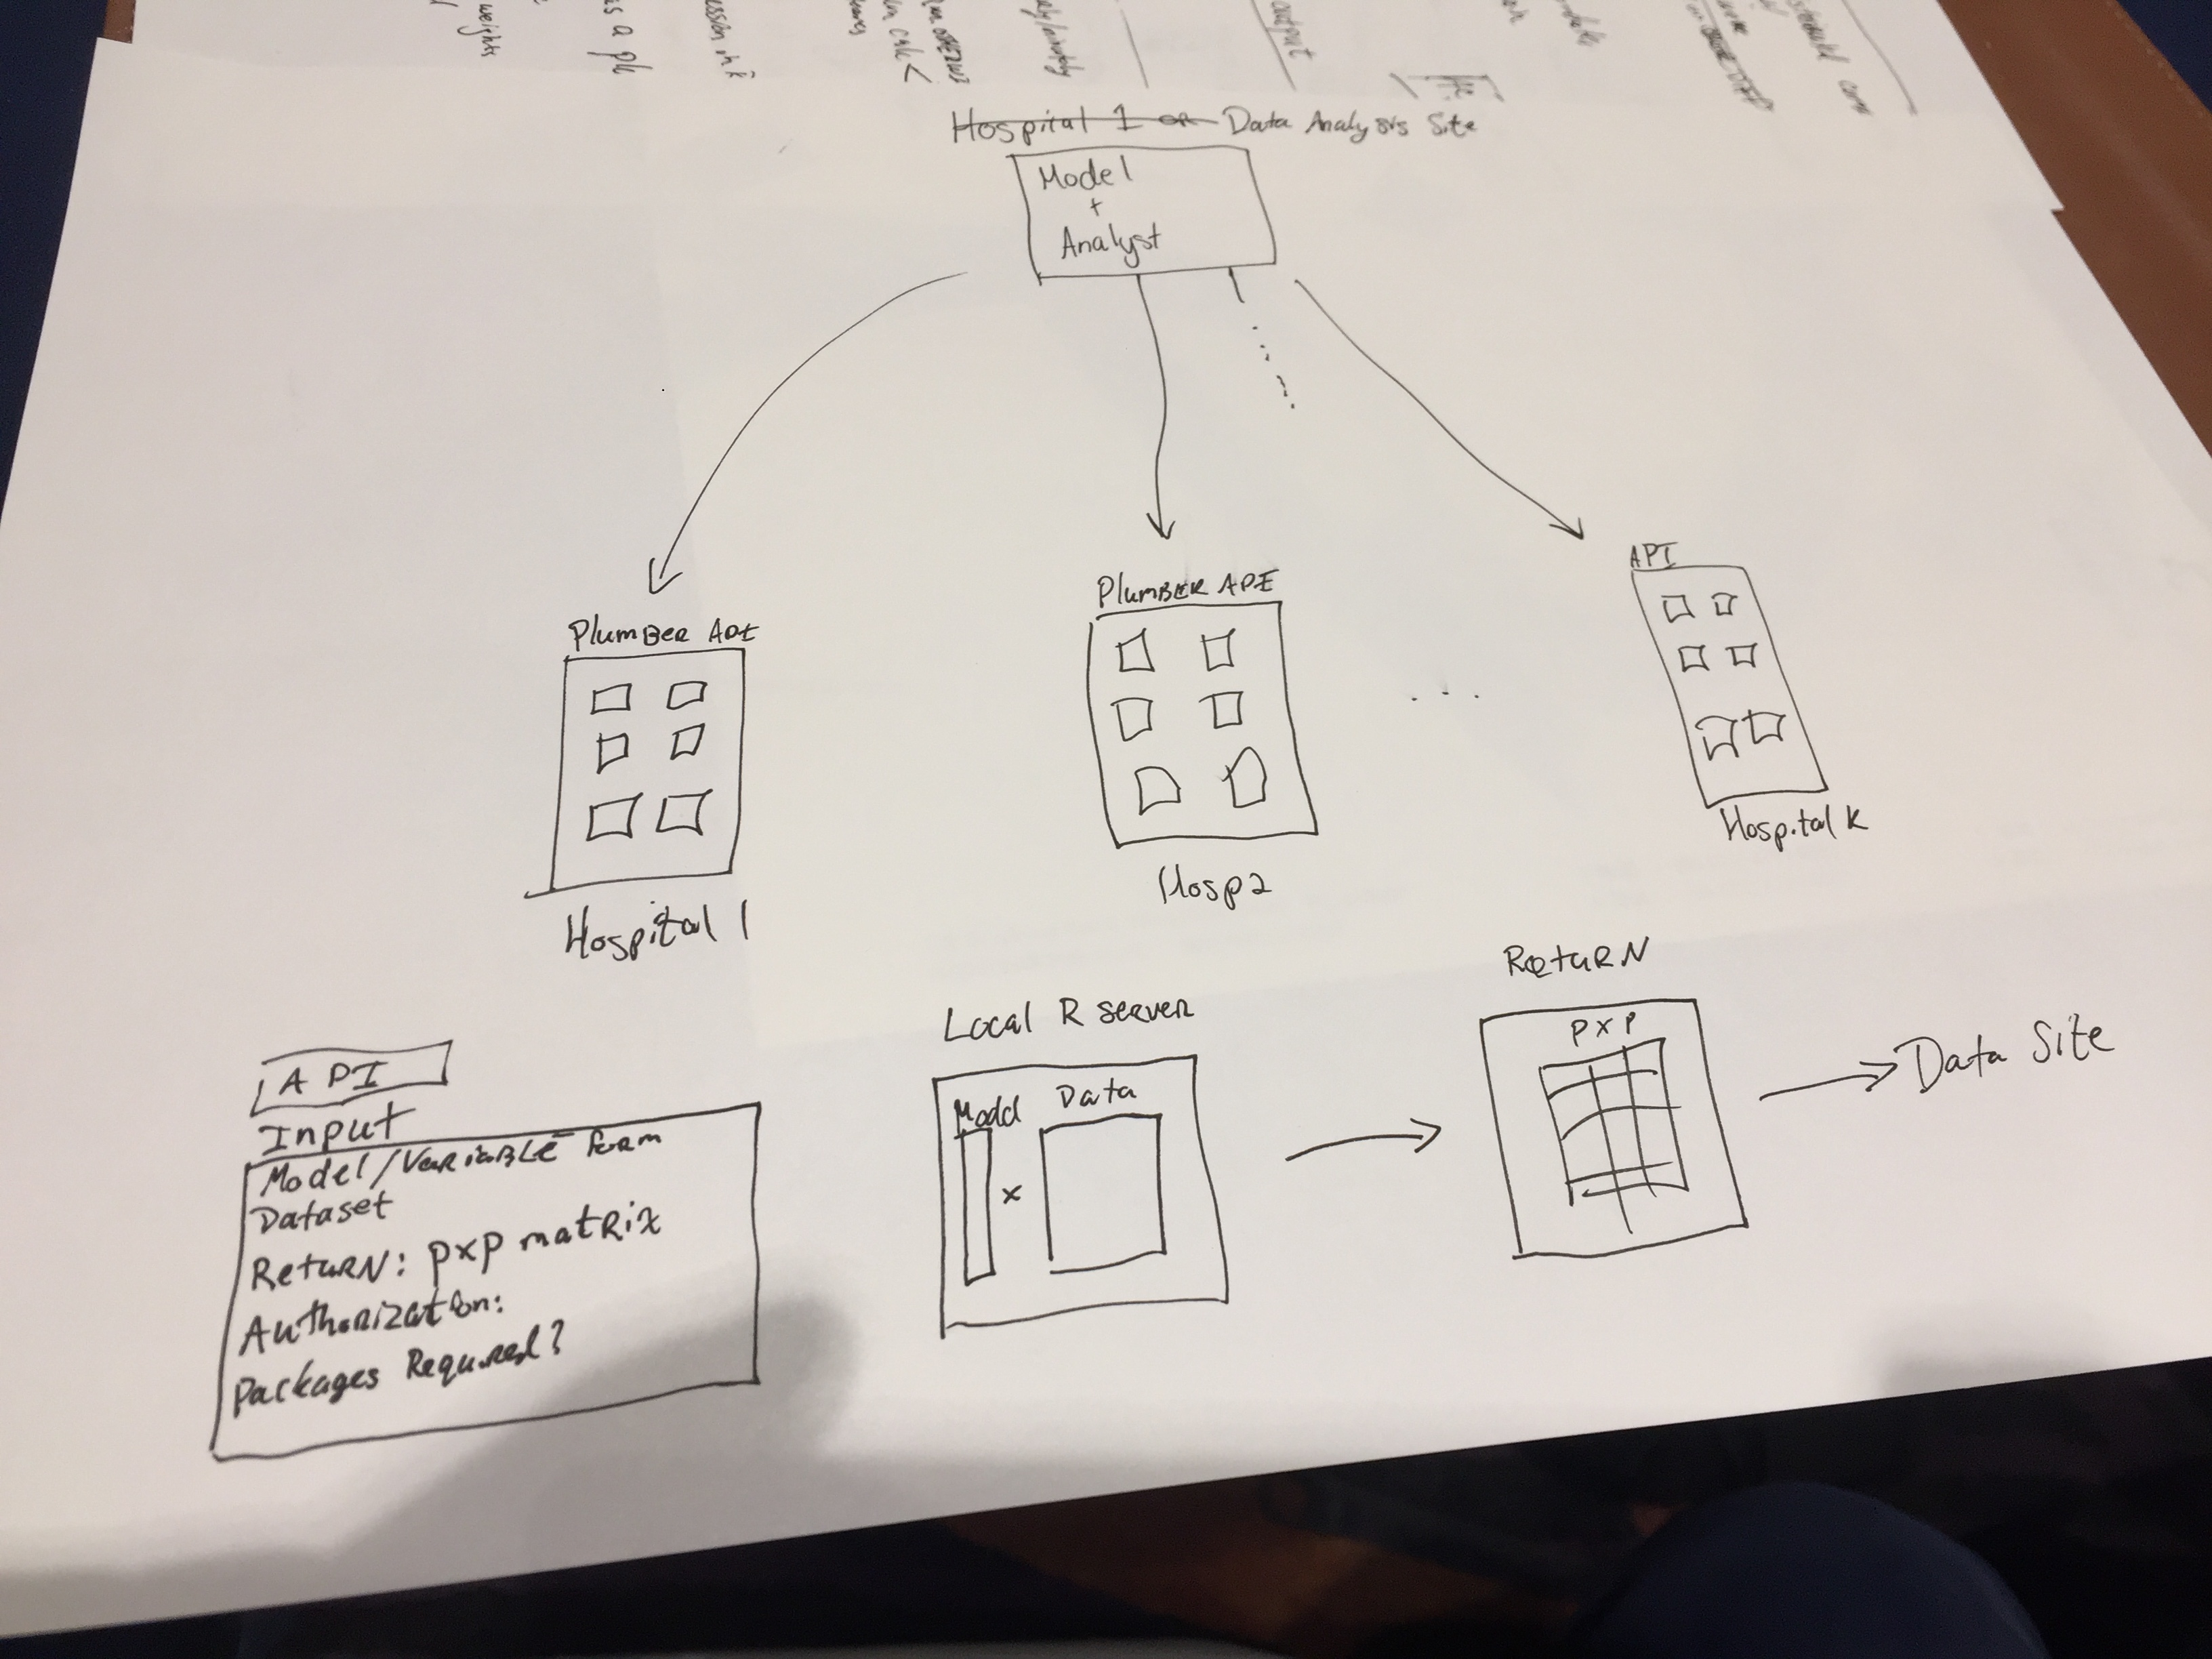
\includegraphics[width=1\linewidth]{sketch} \caption{Proposed Framework.  The modeler/analyst specifies a model, sends the model specification to an endpoint on each hospital API, a computation is run and returned to the analyst and aggregated (usually a gradient).  The model estimates are updated and the process repeats until the model converges.  }\label{fig:unnamed-chunk-1}
\end{figure}

\hypertarget{issues}{%
\section{Issues}\label{issues}}

Though the system may seem simple to describe, many obstacles exist.
Mainly opening any system that interacts with patient data or a database
(even if it were a spreadsheet) is a potential security risk which most
clinical centers will not allow. Though this caution is warranted, it
may be more secure than the alternative of sending estimates in other
communication systems such as email. Though emailing has the upside of a
human ensuring only aggregate data is transferred, it drastically
increases the potential for wrong computation. For example, the
\texttt{plumber} API can have checks on the data for missingness,
quality, the sample size is equal to that of the previous
iteration/model, and other issues, which may be done at varying levels
at each institution.

If the institution allows the API to be supported, then a server is
required, and usually an administrator to oversee it. This administrator
is usually trained in information systems or information technology,
which is likely not part of the clinical team. Thus, providing support
or interaction from the clinical team to the technical personnel can be
more costly than simply emailing estiamtes. Lastly, many institutions
and research groups would like a ``handle'' on what models are being fit
with their data, and thus limits on the API need to be created, which
may cause other issues or limitations on teh proposed framework.

These downsides are vastly outweighed when the API gets repeated use.
Thsu, fitting one model one time does not generally warrant the work
needed to set up this framework.

\hypertarget{references}{%
\section*{References}\label{references}}
\addcontentsline{toc}{section}{References}

\hypertarget{refs}{}
\leavevmode\hypertarget{ref-duncan1980approximate}{}%
Duncan, G.M., 1980. Approximate maximum likelihood estimation with data
sets that exceed computer limits. matrix 2, 1.

\leavevmode\hypertarget{ref-mcdonald2009efficient}{}%
Mcdonald, R., Mohri, M., Silberman, N., Walker, D., Mann, G.S., 2009.
Efficient large-scale distributed training of conditional maximum
entropy models, in: Advances in Neural Information Processing Systems.
pp. 1231--1239.

\leavevmode\hypertarget{ref-plumber}{}%
Trestle Technology, LLC, 2018. plumber: An API generator for R.

\leavevmode\hypertarget{ref-zinkevich2010parallelized}{}%
Zinkevich, M., Weimer, M., Li, L., Smola, A.J., 2010. Parallelized
stochastic gradient descent, in: Advances in Neural Information
Processing Systems. pp. 2595--2603.


\end{document}


